\chapter{Background}

This thesis is split into two parts that focus on different aspects of relationship extraction in the Czech language. In this chapter, we provide a glossary of some NLP and relation extraction terms, we elaborate on the task itself, and we include an introduction to the Czech language for non-Czech readers.


\section{Terminology}
Terminology in NLP subtasks is often non-standardized or not exact. We attempt to introduce the most important concepts for our work as exactly as possible while respecting the terms that seem to be already established. 


\defineterm{Relation} in this context is an abstraction of a semantic relation, for example, a father relation. A relation has a type (father), it is binary (between a son and the father) and oriented (the father and the son are not interchangeable), and describes the relationship between a subject (the son) and an object (the father). We will use the term relation as an equivalent for its type and the term relationship for an instance of the relation. 



\defineterm{Subject} and \defineterm{Object}. The subject is the first argument of a relation, and the object is the second. In the sentence \vuvozovkachtextit{Albus Severus is Harry Potter's son.} a relation of type \relationtype{son} is captured, the subject is Harry and the object is Albus Severus. The reasoning for this choice of direction is as follows: suppose we are gathering information about Harry, then we would probably have both the information that his son is Albus Severus and that his father is James. So we are gathering information about the subject (Harry Potter), even though in most sentences Harry is likely to be the grammatical object: \vuvozovkachtextit{James is Harry's father.} We will use the notation \relation{relation}{subject}{object}: \relation{son}{Harry Potter}{Albus Severus Potter}. 



Both the subject and the object can generally be any word or sequence of words that represent concepts that can form relations. In some cases, subjects, objects, or both are limited to entities or named entities.

\defineterm{Named entity} is a real-world object, such as a person, location, organization, and products, that can be denoted with a proper name. Named entities can be viewed as instances (e.g., New York City is an instance of a city) of some concept -- \defineterm{class}. Sometimes, numeric data is considered in this category as well (for example, by Named Entity Recognition tools). An \defineterm{entity} is a named entity whose proper name is unknown or unimportant but still is an instance. (The word book can represent an abstract concept - a class - as well as an entity.) 

\defineterm{Relation inventory} is the set of relations that are considered valid for a given dataset or model.

\defineterm{Positive relation mention} is a sentence that captures a relationship: a relation together with a tagged subject and object. We will omit the word \textit{positive} unless we want to emphasize the fact.

\defineterm{Negative mention} is close to a (positive) relation mention in the sense that it is a sentence with tagged subject and object, but the relation type is one of the following types: 
\begin{itemize}
\item \relationtype{other} - human annotator would classify a relation, that is not in the inventory.
\item \relationtype{no relation} - in this case, human annotators should feel an absence of a relationship between the subject and the object.

\end{itemize}

\relationtype{No relation} comes with difficulties. Since there is no semantic relationship between subject and object, it makes it harder to choose subject-object pairs. It is probably desirable to have subject-object pairs that could be related in a different sentence.


\section{Relationship Extraction}
The relationship extraction task concentrates on the prediction of relationships. In the typical setup, the goal is to predict a relation type based on a sentence with two tagged entities. Variations of this exist, for example, in real-life applications, the goal might be to output a set of relationships based on a longer piece of text (and therefore the extractor would have several sentences mentioning the same entities). 

Since the input for a relationship extraction model should contain tagged entities, a pipeline of an entity tagging tool and relationship extraction model would be necessary to perform relationship extraction on real data. 

We are aware of two sources of motivation for relationship extraction. First, it can be an alternative to a summarization tool. Therefore it could be used in situations when people are required to read long texts in a short amount of time. In the second application, the extractor could convert texts into structured data and therefore build a graph of entities and their relations. For both applications, an entity linking tool would be beneficial (such a tool disambiguates named entities to a knowledge base) to eliminate the confusion of similarly named entities.

\label{sec:relation_extraction_pipeline_proposal}
Since many applications are likely to benefit from entity disambiguation, a pipeline of a named entity recognizer, an entity linker and finally a relationship extraction would potentially be useful.

\section{Czech language}
\label{sec:Czech}
One of the objectives of this thesis is to work with the Czech language. Therefore we find it useful to make some notes on Czech (for non-Czech speaking readers). Czech is a Slavic language with rich morphology and relatively free word order. Most of the Czech morphology can be treated with a morphological analyzer. Still, it might be useful to have a better understanding of the language we are working with.

\subsection{Inflexion}
In Czech, nouns, adjectives, pronouns and numerals are declined. The declination expresses (not necessarily unambiguously) one of seven cases and a number (singular or plural). Any inflected word in Czech has grammatical gender. For words that have natural gender, those two genders nearly always align: \vuvozovkach{žena} \preklad{woman} is feminine and \vuvozovkach{muž} \preklad{man} is masculine. The inflexion of each declinable word follows a pattern. This all means that a single word can have relatively many different forms.

Verbs are conjugated, the conjugation expresses person, number, tense, voice, mode and others. Verbs follow one of 14 patterns. An average Czech either finds the theory about Czech verbs and tenses confusing or is even unaware of the existence of the verb patterns. That likely contributes to common use of incorrect forms of verbs even in the official language.

An important aspect of declension for us is agreement. In English, subject and verb agree (limited just to the third person). In Czech, subject and verb also agree, but there also needs to be an agreement in noun phrases. 


\begin{figure}
\centering
\subfloat[Declension of \vuvozovkach{příčný} (diagonal)]{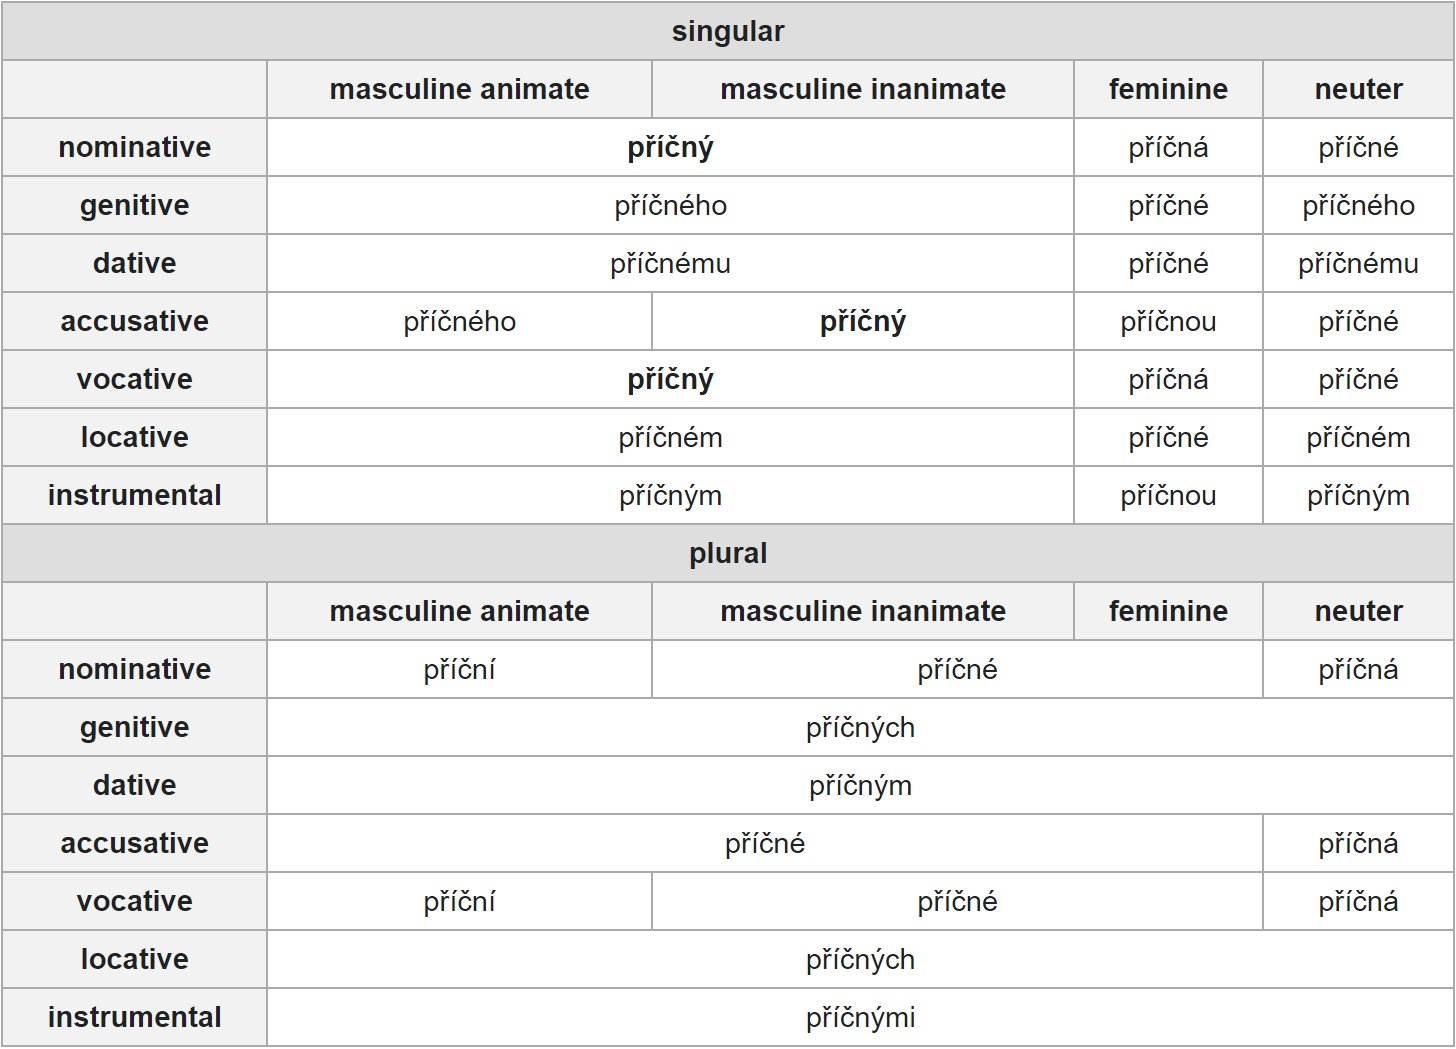
\includegraphics[width=0.95\textwidth]{./img/pricna} \label{obr:pricna}}
\qquad
\subfloat[Declension of \vuvozovkach{ulice} (street)]{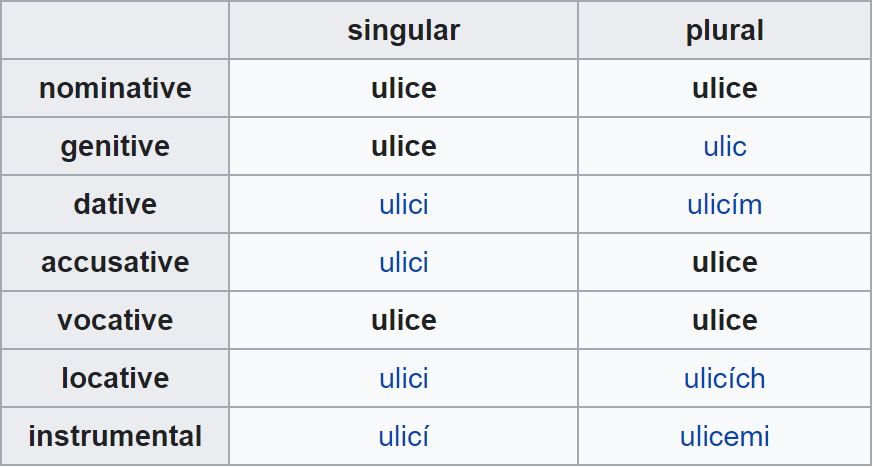
\includegraphics[width=0.60\textwidth]{./img/ulice} \label{obr:ulice}}

\caption{Examples of czech declension, taken from Wiktionary.\label{obr:pricnaUlice}}
\end{figure}


We include an example to help grasp these concepts to readers who do not speak any inflexive language. In \autoref{obr:pricnaUlice} words \vuvozovkach{příčný} (diagonal) and \vuvozovkach{ulice} (street) are declined, the noun phrase \vuvozovkach{Příčná ulice} is the Czech equivalent of the Diagon Alley. The lexeme sizes are 11 and 7, so combinatorically, the noun phrase could have 77 forms. As we explained, in Czech, there is an agreement in noun phrases, and only 9 different forms of the noun phrase \vuvozovkach{Příčná ulice} are valid. 



\subsection{Word Order}
Unlike in English, the sentence structure is relatively relaxed in Czech. The basic sentence structure is of SVO (subject verb object) type, but even when the word order is entirely different, the sentence might still be understandable thanks to the inflected forms of words. At the same time, the word order is not arbitrary; some orderings of words do not form a valid sentence. Those that are valid can carry a considerably different message (with a different emotion or a different emphasis).

The position of attributes tends to be mostly fixed. Some attributes are prepositive, some postpositive, but most of them stay at the same position (within the noun phrase) unless some enumeration is used. If we return to the \vuvozovkach{Příčná ulice} example, we are not able to recollect a sentence, where the reversed order is used.

